% GEOMIRA export: TikZ. One unit is 60bp (80 px on screen).
% Needs \usepackage{tikz} and \usepackage{amssymb}.
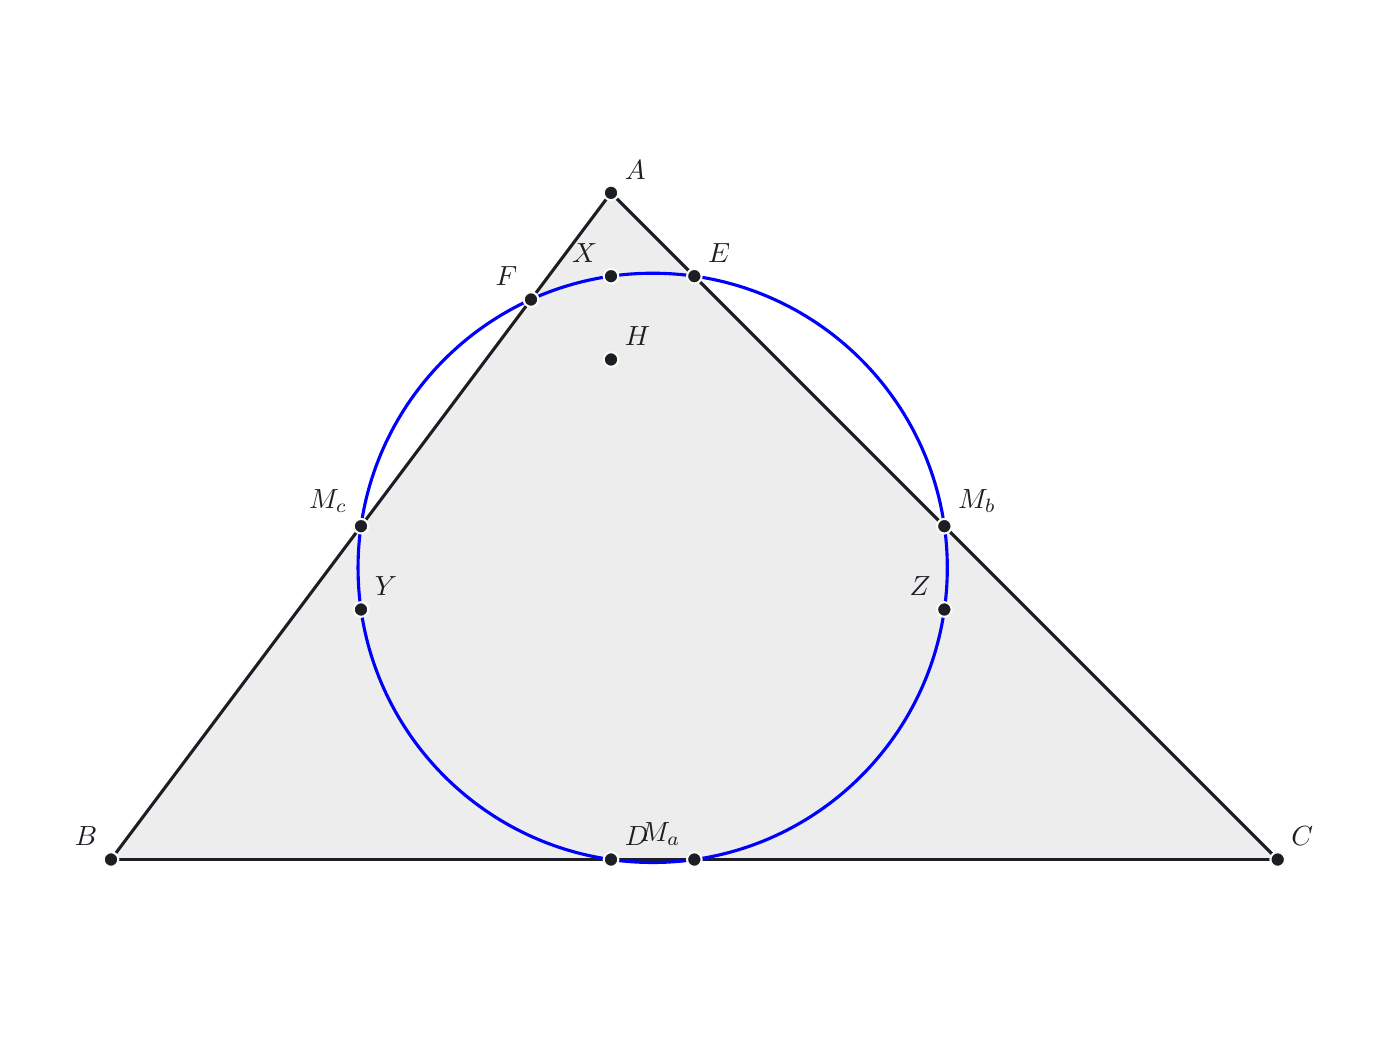
\begin{tikzpicture}[x=60bp, y=60bp, line cap=round, line join=round]
\definecolor{gmc0}{HTML}{1B1F24}
\definecolor{gmc1}{HTML}{0000FF}
\definecolor{gmc2}{HTML}{FBFBF8}
\clip (-2.5,-1.0089) rectangle (5.5,4.9911);
% abc
\fill[gmc0, fill opacity=0.08] (1,4) -- (-2,0) -- (5,0) -- cycle;
\draw[gmc0, line width=1.125bp] (1,4) -- (-2,0);
\draw[gmc0, line width=1.125bp] (-2,0) -- (5,0);
\draw[gmc0, line width=1.125bp] (5,0) -- (1,4);
% ν
\draw[gmc1, line width=1.125bp] (3.0178,1.75) arc[start angle=0, end angle=360, radius=1.76777];
% A
\filldraw[fill=gmc0, draw=gmc2, line width=0.75bp] (1,4) circle[radius=2.625bp];
% B
\filldraw[fill=gmc0, draw=gmc2, line width=0.75bp] (-2,0) circle[radius=2.625bp];
% C
\filldraw[fill=gmc0, draw=gmc2, line width=0.75bp] (5,0) circle[radius=2.625bp];
% H
\filldraw[fill=gmc0, draw=gmc2, line width=0.75bp] (1,3) circle[radius=2.625bp];
% M_a
\filldraw[fill=gmc0, draw=gmc2, line width=0.75bp] (1.5,0) circle[radius=2.625bp];
% M_b
\filldraw[fill=gmc0, draw=gmc2, line width=0.75bp] (3,2) circle[radius=2.625bp];
% M_c
\filldraw[fill=gmc0, draw=gmc2, line width=0.75bp] (-0.5,2) circle[radius=2.625bp];
% D
\filldraw[fill=gmc0, draw=gmc2, line width=0.75bp] (1,0) circle[radius=2.625bp];
% E
\filldraw[fill=gmc0, draw=gmc2, line width=0.75bp] (1.5,3.5) circle[radius=2.625bp];
% F
\filldraw[fill=gmc0, draw=gmc2, line width=0.75bp] (0.52,3.36) circle[radius=2.625bp];
% X
\filldraw[fill=gmc0, draw=gmc2, line width=0.75bp] (1,3.5) circle[radius=2.625bp];
% Y
\filldraw[fill=gmc0, draw=gmc2, line width=0.75bp] (-0.5,1.5) circle[radius=2.625bp];
% Z
\filldraw[fill=gmc0, draw=gmc2, line width=0.75bp] (3,1.5) circle[radius=2.625bp];
\node[anchor=south west, inner sep=0pt, text=gmc0] at (1.0795,4.0795) {$A$}; % label of A
\node[anchor=south east, inner sep=0pt, text=gmc0] at (-2.0795,0.0795) {$B$}; % label of B
\node[anchor=south west, inner sep=0pt, text=gmc0] at (5.0795,0.0795) {$C$}; % label of C
\node[anchor=south west, inner sep=0pt, text=gmc0] at (1.0795,3.0795) {$H$}; % label of H
\node[anchor=south east, inner sep=0pt, text=gmc0] at (1.4205,0.0795) {$M_{a}$}; % label of M_a
\node[anchor=south west, inner sep=0pt, text=gmc0] at (3.0795,2.0795) {$M_{b}$}; % label of M_b
\node[anchor=south east, inner sep=0pt, text=gmc0] at (-0.5795,2.0795) {$M_{c}$}; % label of M_c
\node[anchor=south west, inner sep=0pt, text=gmc0] at (1.0795,0.0795) {$D$}; % label of D
\node[anchor=south west, inner sep=0pt, text=gmc0] at (1.5795,3.5795) {$E$}; % label of E
\node[anchor=south east, inner sep=0pt, text=gmc0] at (0.4405,3.4395) {$F$}; % label of F
\node[anchor=south east, inner sep=0pt, text=gmc0] at (0.9205,3.5795) {$X$}; % label of X
\node[anchor=south west, inner sep=0pt, text=gmc0] at (-0.4205,1.5795) {$Y$}; % label of Y
\node[anchor=south east, inner sep=0pt, text=gmc0] at (2.9205,1.5795) {$Z$}; % label of Z
\end{tikzpicture}
